\section{Introduction}
We are required to extend the capabilities of an implemented RDT(Reliable Data Transfer) model to multiple hosts.

The given model can only communicate with two consecutive hosts, an illustration of this is given in \textbf{Figure \ref{fig:single_host_illustration}}

\begin{figure}[H]\center
 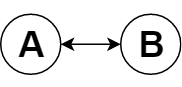
\includegraphics[scale=0.30]{single_host_illustration.png}
 \caption{Single-host illustration}
 \label{fig:single_host_illustration}
\end{figure}


Thus the goal of this project is to communicate across multiple hosts. \textbf{Figure \ref{fig:multi_host_illustration}}
\begin{figure}[H]\center
 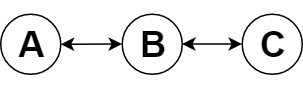
\includegraphics[scale=0.30]{multi_host_illustration.png}
 \caption{Multi-host illustration}
 \label{fig:multi_host_illustration}
\end{figure}


The `host' referenced denotes an entity that can receive and send packets.
